%%
%% This is file `skeleton.tex',
%% generated with the docstrip utility.
%%
%% The original source files were:
%%
%% nuthesis.dtx  (with options: `skeleton')
%% 

%%
%% For common degrees, you can use the class options:
%% phd, edd, ms, ma
%% phd is the default
\documentclass[print]{nuthesis}

\usepackage{graphicx}
\graphicspath{{./images/PNG/}}


\begin{document}
%% Start formatting the first few special pages
%% frontmatter is needed to set the page numbering correctly
\frontmatter

\title{Tweether: A Visualization Tool Displaying Correlation of \\Weather to Tweets}
\author{Shruti Daggumati}
\adviser{Dr. Honfeng Yu}
%\adviserAbstract{Someone}
\major{Computer Science}
\degreemonth{May}
\degreeyear{2015}
%%
%% For most people the defaults will be correct, so they are commented
%% out. To manually set these, just uncomment and make the needed
%% changes.
%% \college{Your college}
%% \city{Your City}
%%
%% For most people the following can be changed with a class
%% option. To manually set these, just uncomment the following and
%% make the needed changes.
\doctype{Project}
\degree{Master of Science}
\degreeabbreviation{M.S.}
%%
%% Now that we know everything we need, we can generate the title page
%% itself.
%%
\maketitle
%%
%% You have a maximum of 350 words for your abstract, which includes
%% your title, name, etc.
%%
%% Required
\begin{abstract}
As the generation of social media we can instantly express how our day is going; however, unknowingly the weather can play a key role in how we are feeling. The weather dictates our lives regardless of what may be happening. The relationship between weather and mood has been immensely studied to show that the weather does play a major factor regarding our emotions. However, how much weather affects us and how we display the relationship using social media remain interesting questions. Based on the natural correlation between weather and mood we propose \emph{Tweether}, a real-time weather and tweet visualization, to see how Twitter users are feeling. This visualization displays a current reflection of emotions in a set of select geographic regions and also predicts possible emotions in these regions in response to the weather forecast. The visualization uses multiple layers to show the connection between locations, weather, and emotions. By aggregating multiple users with similar emotions, we create an aesthetic design that is relatively free of visual clutter and is simple to understand in a 3D manner.
\end{abstract}

%% Optional
%% \begin{copyrightpage}
%% \end{copyrightpage}

%% Optional
%% \begin{dedication}
%% \end{dedication}

%% Optional
%% \begin{acknowledgments}
%% \end{acknowledgments}

%% Optional
%% \begin{grantinfo}
%% \end{grantinfo}
%% The ToC is required
%% Uncomment these if need be

%% The ToC is required
\tableofcontents
%% Uncomment these if need be
%\listoffigures
%\listoftables
%%
%% ``Real'' beginning of the document.
%% mainmatter is needed to set the page numbering correctly
%%   mainmatter is needed after the ToC, (LoF, and LoT) to set the
%%   page numbering correctly for the main body
\mainmatter

%% Thesis goes here


\firstsection{Introduction}
\maketitle
%% \section{Introduction} %for journal use above \firstsection{..} instead

Weather affects our daily lives, from what we wear, what activities we do, what type of transportation we use, what we eat, or even how we feel. With the increasing accuracy of weather forecasts, people can gain an idea on the type of weather they can expect for upcoming days. Activities are usually planned according to the weather outside (e.g., weddings) and alternative plans must be made in case of inclement weather. How people dress is also affected by weather; when the temperature drops people need to wear coats to stay warm. The economy is also greatly affected by the weather. Certain weather conditions can lower crop yield and cause higher prices in stores. Disastrous weather phenomena such as hurricanes, tornadoes, or even floods can cause devastation in communities resulting in homelessness, death, and destruction. Inclement weather can also cause delays in transportation on roads or via flights. We can also choose to ride our bike to work instead of driving the car if the temperature is warm enough. One thing that is an effect of all these items is how we feel.
%----------------------------------------------------------
\begin{itemize}
\vspace{-.1in}
\setlength{\topsep}{-0.1in}
\setlength{\itemsep}{-0.05in}
\item Are you sad that you cannot enjoy the outdoors due to rain?
\item Do you love that it's raining so you can bundle up and read your favorite book?
\item Do you love the snow because it's close to Christmas?
\item Do you hate the winter because you want it to be spring?
\end{itemize}
\vspace{-0.05in}
%----------------------------------------------------------
These feelings are all brought out by the weather outside. One person can feel positive about a certain type of weather and one person can feel negative. In this work, we showcase a novel tool, named \emph{Tweether}, a visualization of real-time Twitter and weather data to show the feelings of current users and how their emotions could fluctuate. Having the weather forecast %up to 72 hours
in the future, the emotions in current regions can be predicted.

We see if the weather has any correlation to the majority of the population and we try to predict the future feelings of given weather. For example, when thinking about warm and sunny weather we naturally assume the majority of the population will be happier in comparison to dreary or cold temperatures. We plan to examine if the majority of the population follows such patterns. We will also examine how the overall sentiment changes when we filter tweets so only tweets in regards to weather are displayed.

It is not enough to just determine the correlation between emotion and weather, but a novel visualization is necessary. Our work showcases a 3D map which highlights select clusters of weather. The correlation of tweets to weather is represented by a graph. We use line bundling to visualize the graph to reduce visual clutter. Introducing a clear relationship between weather and tweets, the design presents a natural manner of representing correlation. 
\section{Related Work}

Visualizations correlating sentiment and weather are highly sparse, and the presence of live visualizations is also non-existent. However, there are works showing the two portions of this work. Clustering of weather data has been done many times in the past. There is also a vast number of visualizations which indicate the sentiment of different locations.

\subsection{Psychological Studies}

The natural correlation of weather with emotion has been studied profusely~\cite{denissen2008effects,howarth1984multidimensional,keller2005warm,lambert2002effect}. With various factors among the different research, the conclusions attained were broad. In general, humidity, sunshine, and temperature have the greatest effect on mood~\cite{howarth1984multidimensional}.

In some research on weather and mood, correlations have been debunked. There is no consistency due to seasons and time spent outside~\cite{keller2005warm}. Having certain emotions regarding the season has strong links to seasonal affective disorder (SAD), where people are depressed in regards to changes of the seasons, which usually occurs during the winter. However, most psychologists believe that the weather has an impact on psychological intentions~\cite{denissen2008effects}. When observing serotonin levels in regards to sunshine there were strong relationships to being happy~\cite{lambert2002effect}. It has been found that weather may not play a big role in the positive attitude, but the negative attitude can have a correlation with weather~\cite{howarth1984multidimensional}.


\subsection{Social Media, Weather, and Emotions}

When dealing with the correlation of weather with emotion the research is fairly sparse. Few works present the use of Twitter data for their social media feed and some form of weather data. However in comparison to our work the following research used past data and developed a 2D graph implementation for visualization.

Work has been done using two to four years of Twitter data and correlating it with meteorological data from NOAA~\cite{hannak2012tweetin,li2014nasty}. Using urban areas in the United States as the area of interest, the tweets are passed to a sentiment analyzer that has a multi-level process. The researchers first determine keywords which are identified from public events (e.g., entertainment or natural disasters), they then identify the mood state, and finally assign sentiment scores. To correlate the weather with the tweets they use a Generalized Mixed Model to display the non-linear relationship between emotion and weather. Using multiple variables for weather (temperature, temperature change, precipitation, snow depth, wind speed, solar energy, and hail), they determine the connection to hostility-anger, depression-dejection, fatigue-inertia, and sleepiness-freshness. Their results indicate that the warmer temperatures create an angrier atmosphere, lower depression, and less sleepiness, and they determine the influence of temperature to mood is trivial. Their visualization is limited to graphs. Other than using urban areas in USA the researchers see relationships between temperature, humidity, and atmospheric pressure for tweets in the United States and weather data from Weather Underground ~\cite{park2013mood}. Using Linguistic Inquiry and Word Count for sentiment classification they see a pattern with temperature and emotion of every state in the United States. Using regression analysis they find that the warmer states have a happier mood than the colder states. Their visualization is limited to a bar chart.

These works are limited in visualization and usability study. Using past data is useful for our training and testing model; however, having a live view of what Twitter users feel is what we aim for in this work.


\subsection{Sentiment Analysis in Social Media}

Sentiment analysis has been studied vastly. There are various methods to detect the sentiment of a sentence. However, in regards to tweets sentences may be incomplete, because a tweet is limited to 140 characters and the need to express oneself is limited to short meaningful phrases. We find abbreviations, neologisms, acronyms, hashtags, emoticons, and URL's throughout most tweets.

Certain features need to be extracted and some need to be filtered out. Filtering of URL's, usernames, Twitter special words, and emoticons may be needed in certain scenarios~\cite{pak2010twitter}. Stop words (i.e., a, an, the, etc.) are also removed due to not adding any extra sentiment information. For classifying the tweets, a number of different methods are used, and the most prevalent one is the Naive Bayes classifier~\cite{pangthumbs}. Emoticons are used as basis for sentiment classification for classifying tweets as positive or negative for the training purposes~\cite{keller2005warm,agarwal2011sentiment}.

Using emoticons for classifying training data is novel; however, most tweets gathered in the live feed have a very low count of emoticons. Thus, emoticons are not employed in our method. Filtering of URL's and usernames is used for our method. We also add the filtering process to drop phrases beginning with hashtags.

\subsection{Visualizations}

\subsubsection{Clustering}

Although clustering of data has been extensively studied, it remains a non-trivial task to deal with temporal and time series data. Weather data needs to be clustered based on values, proximities, and changes throughout the given time span. There have been various visualization techniques for time series data. Visualizing time series data using spirals for large data sets can better identify periodic structures in data~\cite{weber2001visualizing}. Using wavelet to transform data along a multi-resolution temporal representation to find clusters with similar trends is a useful method for exploring data in a time series fashion~\cite{woodring2009multiscale}. Applying smooth data histograms for visualizing clusters in self-organizing maps is a simple method for 2D data sets~\cite{pampalk2002using}.

The mass majority of clustering visualizations uses k-means clustering on the basis of their algorithms~\cite{weber2001visualizing,woodring2009multiscale,pampalk2002using}. We choose to follow this pattern as well, as K-means is a widely chosen algorithm that gives reasonably good results ~\cite{weber2001visualizing,jain2010data}.

\subsubsection{Bundling}

The correlation between multiple entities (e.g., various weather and emotion patterns in our study) can be fundamentally represented as a graph. However, graph visualization remains a challenging task. Severe visual clutter can be easily incurred if we directly draw all edges as straight lines, even with some optimization techniques, such as force-directed placement of vertices or clustering of vertices~\cite{KAUFMANN2001}.

To address this issue, Holen~\cite{holten2006hierarchical} proposed a concept of \emph{edge bundling} that groups the related edges of a hierarchical graph together as a set of smooth curved bundles, and thus can significantly reduce visual cluster. Holen et al.~\cite{holten2009force} extended the original edge bundling method and presented force directed edge bundling (FDEB) for a general graph without hierarchy. Other researchers have also made similar efforts to generalize edge bundling~\cite{cui2008geometry,telea2010image,ersoy2011skeleton,gansner2011multilevel}. Few efforts have been dedicated to creating extensions in 3D space. Lambert et al.~\cite{5571244} presented a 3D edge bundling to visualize geographical networks on the Earth surface. B\"{o}ttger et al.~\cite{bottger2014three} presented mean-shift edge bundling to visualize 3D functional connectivity across the cortical regions of the brain. Their method combines FDEB and kernel density estimation edge bundling (KDEEB)~\cite{hurter2012graph} with an improved numerical stability.

\subsection{Predictions}

Using the past Twitter data set, it is necessary to predict the mood for the next days. Predicting the stock market based on Twitter mood has been studied~\cite{bollen2011twitter}. The notion that the mood of Twitter users can correlate to stocks immediately is not present; however, the mood is reflected when a few days have passed. Because the general public has strong connections with the outcome of a man-made entity, there will be some form of correlation available. In our case, however, the weather is not a man-made entity. Thus, finding a correlation between weather and mood, and then predicting the mood for the future can show zero correlations. We will address this idea later in this paper.

\chapter{Approach}

Implementing Tweether has multiple steps which are composed of individual and interconnected components. We use both the weather data and the Twitter data in our study (Section~\ref{sec:dataset}). Based on the clustering result of the weather data (Section~\ref{sec:clust}) and the sentiment classification of each tweet (Section~\ref{sec:senti}), we correlate these two entities (Section~\ref{sec:corr}). We also predict the sentiments for future times (Section~\ref{sec:pred}).

Tweether in its simplest form takes tweets and assigns a sentiment value which is then correlated to the nearest weather cluster. Each tweet is aligned to the map according to its geographic location. The current hour visualization and the prediction visualization have the same user interface. We represent the derived correlation as a graph, and embrace the natural link of weather up in the sky to the tweets down on the ground to implement our visualization (Section~\ref{sec:vis}). After we implement each of the necessary steps we can clearly see how the visualization adopts a layered design which effectively highlights the correlation of weather and emotion in space-time. The major steps of Tweether are illustrated in Figure~\ref{fig:steps}.

%----------------------------------------------------------
\begin{figure}[t]
 \centering
 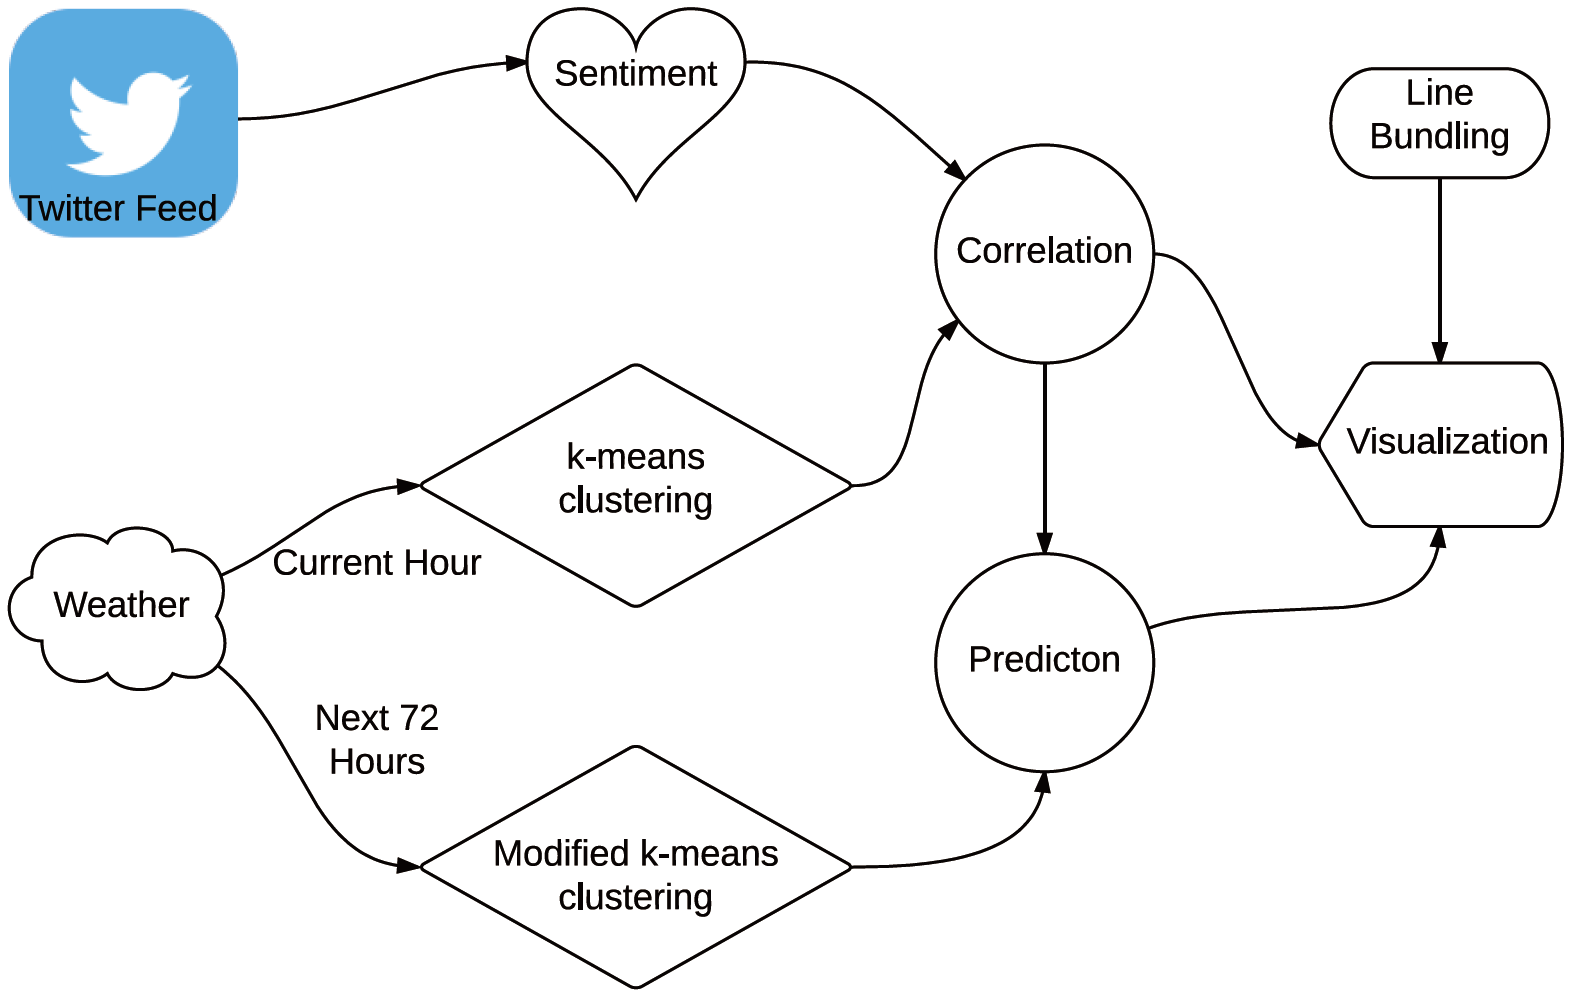
\includegraphics[width=0.75\linewidth]{steps}
 \caption{The major steps of Tweether.}
 \label{fig:steps}
\end{figure}
%----------------------------------------------------------


%We describe the different data sets we used in Section~\ref{sec:dataset}, how we clustered the weather data in Section \ref{sec:clust}, and how we predicted the sentiment of each tweet in Section \ref{sec:senti}. Correlating the two entities of this work is described in Section \ref{sec:corr}, and the implementation of the line bundling to indicate the correlation in Section \ref{sec:line}.  In addition to these items, we try to implement a prediction  for the sentiment for future times which we discuss in Section \ref{sec:pred}. The steps are illustrated in Figure \ref{fig:steps}.

\section{Data Sets}
\label{sec:dataset}

We use two main data sets with respect to weather and Twitter in this work. The weather data set is generated from a climate simulation using Weather Research and Forecasting (WRF) Model~\cite{Michalakes2004}. %from the Holland Computing Center (HCC).
The data provides hourly forecasts with up to 72 hours in the future. Each WRF file contains multiple variables in regards to weather (i.e., temperature, precipitation, wind speed, etc.). For this visualization, we choose to focus on the surface skin temperature (TSK) variable. Each TSK file is represented via a 2D array %$34 \times 24$
covering a regular geographic region. In this work, we use a WRF data that geographically corresponds to the state of Nebraska.
%The WRF file geographically corresponds to Nebraska and surrounding states as seen in Figure \ref{fig:maps}.

The Twitter data set contains the live data feed from Twitter users throughout Nebraska. The fetched Twitter data is synchronized with the weather data. Only users that have opted-in to turn on the feature of Tweeting With Location are selected. In addition, because Nebraska has a fairly low population with most of the land being barren, only the most populous cities are chosen. These cities include Omaha, Lincoln, Grand Island, Kearney, Fremont, North Platte, Norfolk, Columbus, and Scottsbluff. We use a geographic filtering process to select these cities. The Twitter data is stored in JSON format where we need to extract the coordinates of each tweet and the tweet itself. Due to some cities being on the border of Nebraska (such as Omaha), the Twitter data needs to have a second filter which removes any tweets that do not have any relation with Nebraska.

%----------------------------------------------------------
%\begin{figure}[htp]
%  \centering
%  \subfigure[Map showing surrounding states with counties]{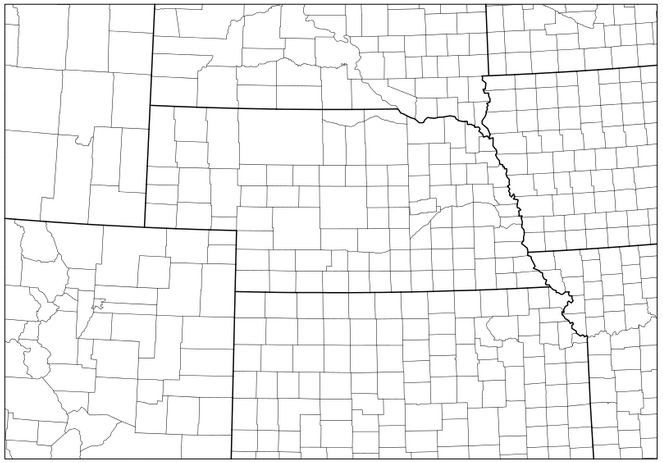
\includegraphics[scale=0.17]{mapBefore}}\quad
%  \subfigure[Map reduced to show prominance to Nebraska]{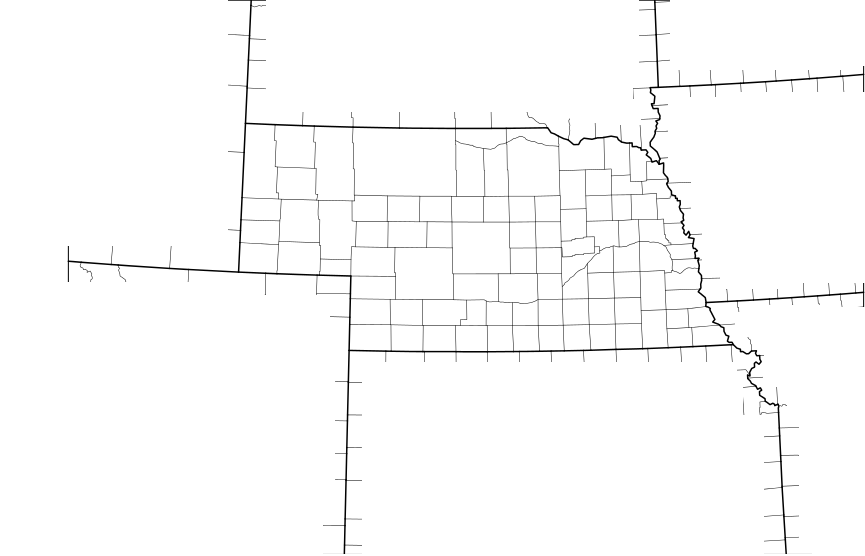
\includegraphics[scale=0.14]{mapAfter}}
%\caption{Nebraska map before and after}
%\label{fig:maps}
%\end{figure}
%----------------------------------------------------------

\section{Weather Clustering}
\label{sec:clust}

We use clustering to extract different weather patterns from the WRF data and identify their geographic coverage. The clustering of weather differs depending on if looking at the current hour or the predicted values for the next 72 hours. For the current hour of weather, we use the k-means clustering algorithm. For the forecasted weather, we use a modified k-means algorithm.
%Since we don't need to worry about the future at the current state nothing additional is added to the algorithm.
%For the forecasted weather, we use the dynamic time warping (DTW) algorithm~\cite{salvador2007toward}.

We use the k-means clustering algorithm to partition the 2D array of each time step of TSK into a set of clusters. Some clusters can be dispersed, resulting in random patterns or outliers. These outliers are removed because we assume that moods are affected mostly by comparably dominant weather patterns, and the outliers are small in space and can be changed dynamically in time. To remove outliers, we use a filtering process based on the number of data points in each cluster. If there exists a cluster which has less than one percent of the overall number of clustered elements, this cluster is removed and the data points which belong to a cluster are clustered again. This process is continued until there is no cluster which has less than one percent of the overall cluster count. For the forecasted weather, we use a modified k-means algorithm, where we use the difference between two successive hours for the similarity measures.

%In this study, we choose five clusters that gives us good results.
%
%For the forecasted weather, we used DTW to measure the similarity between two successive hours, because k-means is not very robust towards outliers due to adding a square weight on the value.

%For the forecasted weather, we used DTW to measure the similarity between two successive hours.
%, because k-means is not very robust towards outliers due to adding a square weight on the value.

To smooth any randomness in the cluster values of the 2D array, we use a low-pass filter where the cluster value of an element is determined by the values of surrounding elements.
%connectivity is used to determine the percentage of surrounding elements with the same cluster value as the central element.
If at least 5 out of 8 neighbors have the same value, the cluster values of the element is kept; otherwise, the value is removed. We found that repeating this operation 4 times can give us sufficient smooth outcome amongst the majority of 72 hours.
%The number of times to be repeated is chosen due to it creating the most smooth outcome amongst the majority of 72 hours. Figure~\ref{fig:clustering} (d) shows the result of forecasted weather.
Figure~\ref{fig:clustering} (a) shows the distribution of TSK at a certain time step. A direct use of k-means can generate many dispersed small regions, as shown in Figure~\ref{fig:clustering} (b). Our method can clearly extract the dominant TSK patterns, as shown in Figure~\ref{fig:clustering} (c). Figure~\ref{fig:clustering} (d) shows the result of the forecasted weather.

%------------------------------------------------
\begin{figure}[t]
\begin{center}
$\begin{array}{c@{\hspace{0.01\linewidth}}c}
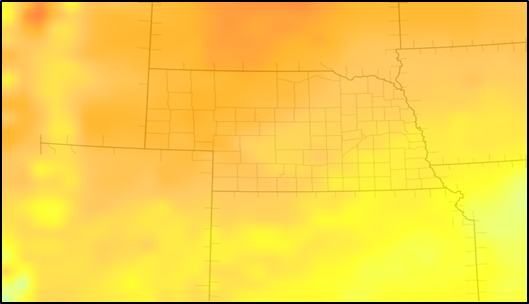
\includegraphics[width=0.49\linewidth]{clustering_raw} &
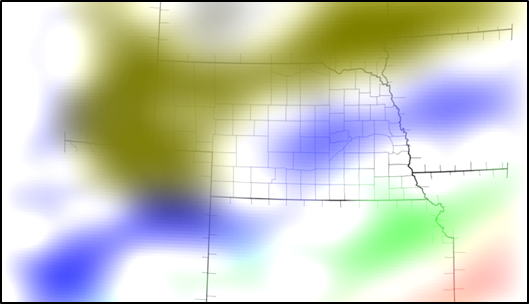
\includegraphics[width=0.49\linewidth]{clustering_org}
\\
\mbox{\small{(a)}} & \mbox{\small{(b)}}
\\
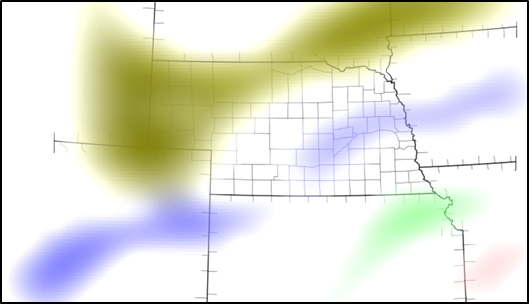
\includegraphics[width=0.49\linewidth]{clustering_smooth} &
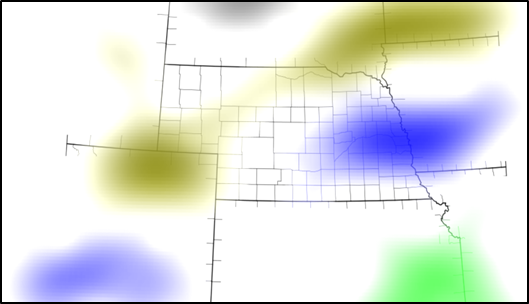
\includegraphics[width=0.49\linewidth]{clustering_time}
\\
\mbox{\small{(c)}} & \mbox{\small{(d)}}
\end{array}$
\end{center}
\vspace{-.1in}
\caption{(a) The geographic distribution of TSK variable at a time step. (b) The k-means result with outliers. (c) The comparably dominant weather patterns. (d) The clustering result of forecasted weather using the modified k-means clustering. The color values in (a) are mapped to TSK. The color values in (b)-(d) are used to distinguish different clusters.}
\label{fig:clustering}
\end{figure}
%------------------------------------------------

\section{Sentiment Classification}
\label{sec:senti}

Each tweet can contain different attributes other than plain sentences. Due to each tweet being limited to 140 characters, the majority of users tend to use abbreviations, neologisms (e.g., noob, troll), acronyms hashtags, emoticons, or URL's. Abbreviations, acronyms, and neologisms are taken into account for training our classifier. However, a few items are filtered from certain tweets. The filtering process removes emoticons, URL's, usernames, and hashtags. In some situations, it is known that hashtags can provide instant insight as to what the users are feeling~\cite{agarwal2011sentiment}. However, most hashtags that we encountered contain meaningless text or sentences for tags instead of keywords.

We use the Naive Bayes classifier~\cite{pak2010twitter} to determine the sentiment of tweets. Robert Plutchik's theory~\cite{Plutchik2002} states that there are eight basic emotions within two categories:
%----------------------------------------------------------
\begin{itemize}
\vspace{-0.05in}
\setlength{\topsep}{-0.1in}
\setlength{\itemsep}{-0.05in}
\item negative - fear, anger, sadness, depression, disgust
\item positive - joy, trust, anticipation, surprise
\end{itemize}
\vspace{-0.05in}
%----------------------------------------------------------
These emotions are the basic training portion of the classification of tweets. The synonyms for each category are taken into account and this sets up the basic foundation for the tweet classifier.

Other than acronyms we also need to take into account profanity. The use of profanity in social media is very high and it may lead to a positive or negative emotion depending on the situation. To take into account how profanity is used in sentences, we fetched tweets to explore the usage of these words. We found that using these tweets to train the classifier gave a high accuracy rate in regards to profanity. In the beginning, we tried to remove any tweet with profanity, however, this drastically lowered our tweet count. We then tried to remove the occurrences of profanity in the tweet and used the remaining words as a judge of emotion, but this only worked in a few cases. For the majority of these tweets, we believe that profanity gave insight to negative moods and thus decided to take into account profanity.

Due to tweets using abbreviations and incomplete sentences, sentiment calculation is a non-trivial task. The classifier is trained using around 10,000 tweets, where each tweet is given a positive or negative score, and there were rare occurrences of duplicate tweets. There is an equal portion of positive and negative tweets in regards to words where sentiment could go either way. Figure~\ref{fig:sentiment} shows the sentiment classification results of two time steps.

%------------------------------------------------
\begin{figure}[t]
\begin{center}
$\begin{array}{c}
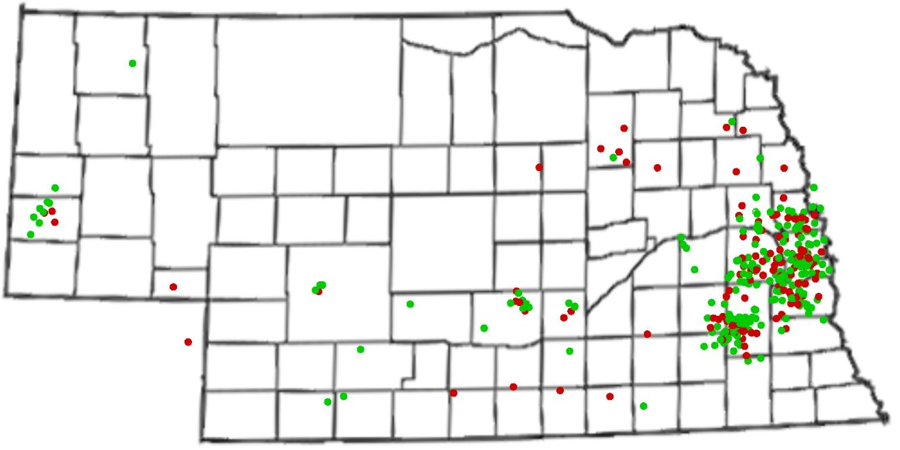
\includegraphics[width=0.9\linewidth]{sentiment_t1} \\
\mbox{\small{(a)}} \\
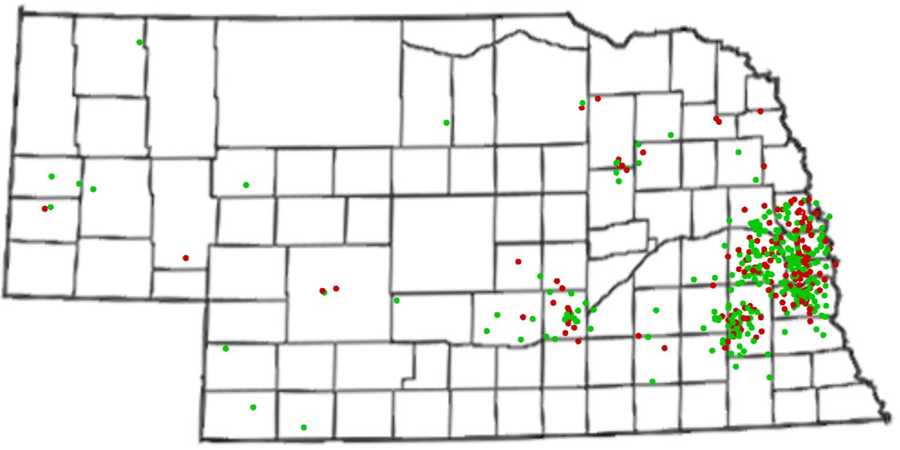
\includegraphics[width=0.9\linewidth]{sentiment_t2} \\
\mbox{\small{(b)}}
\end{array}$
\end{center}
\vspace{-.1in}
\caption{The sentiment classification results and their geographic distribution of two time steps over Nebraska, where a green point corresponds to a tweet with positive sentiment and a red point corresponds to a tweet with negative sentiment.}
\label{fig:sentiment}
\end{figure}
%------------------------------------------------


\section{Correlation}
\label{sec:corr}

We investigate the correlation between the patterns generated by the weather clustering and the sentiment classification. These patterns are characterized with geographic distributions. Figure~\ref{fig:correlation} (left image) illustrates an example of two tweets, $T_1$ and $T_2$, and four weather clusters, $W_1$, $W_2$, $W_3$ and $W_4$. It is intuitive that the sentiment derived from a tweet is mostly affected by its overlapped weather cluster. We call such a cluster as the \emph{primary} cluster of a tweet. If there is a naturally geographic overlap between a tweet and a weather cluster, the mapping is pure, such as $T_1$ and $W_1$ in Figure~\ref{fig:correlation}. In situations where there is no direct overlap for a tweet to any of the weather clusters the nearest cluster is used, such as $T_2$ and $W_1$ in Figure~\ref{fig:correlation}.

%The correlation between each tweet and the cluster above is represented by a one to one mapping. As we see in Figure \ref{fig:clusters}(a), if there is a natural link then the mapping is pure. In situations where there isn't a direct link to any of the weather clusters the nearest cluster is used.

Other than the natural link between the primary cluster and a tweet, we explore the similarity of connections of the tweet to other clusters. % regardless of the sentiment it may correspond to.
This is because the sentiment of the tweet can be also affected by its vicinal weather clusters. Therefore, disregarding the primary cluster, we quantify the correlation of the tweet to the other clusters to indicate what other clusters the tweet could map to. In particular, we use the location of a tweet and the TSK value at the location to determine the correlation value to the points of a weather cluster using the Pearson product-moment correlation coefficient:
%------------------------------------------------
\begin{equation}
\label{eq:pearson}
\rho_{X,Y}=\frac{cov(X,Y)}{\sigma_{X}\sigma_{Y}},
\end{equation}
%------------------------------------------------
where $X$ is the location and the TSK value of the tweet, $Y$ is the locations and the TSK values of all points of a weather cluster, $cov$ is the covariance, and $\sigma_{X}$ ($\sigma_{Y}$) is the standard deviation of $X$ ($Y$). The correlation value of $\rho_{X,Y}$ ranges from -1 to 1. If the value is 1 (-1), it indicates a perfect positive (negative) linear relationship between $X$ and $Y$. If the value is 0, it means that there is no linear relationship between $X$ and $Y$.

This correlation is computed for the current hour. For each tweet, we use the top two values of correlation to other clusters which we deem the \emph{secondary} and \emph{tertiary} clusters, respectively. The secondary and tertiary mapping have the same sentiment since the best fit is a cluster close by with a similar TSK value. Figure~\ref{fig:correlation} illustrates the primary, secondary and tertiary clusters of $T_1$ and $T_2$ respectively.

%\marginnote{\pin{why?}}\pin{With a correlation value closer to 1 we keep the sentiment expressed in the primary cluster. However, in the case of a correlation value closer to -1, we swap the sentiment expressed in the primary cluster. We look for the values closest to 1 or -1, and assign the proper sentiment value according to the sign.}


%------------------------------------------------
\begin{figure}[t]
\begin{center}
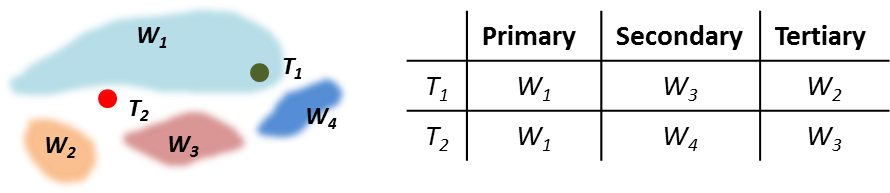
\includegraphics[width=1.0\linewidth]{correlation}
\end{center}
\vspace{-.1in}
\caption{The correlation between the tweets, $T_1$ and $T_2$, and the weather clusters, $W_1$, $W_2$, $W_3$ and $W_4$. The left image shows the geographic distribution of the tweets and the weather clusters. The right table shows the primary, secondary, and tertiary weather clusters of $T_1$ and $T_2$.}
\label{fig:correlation}
\end{figure}
%------------------------------------------------

%%------------------------------------------------
%\begin{figure}[htp]
%  \centering
%  \subfigure[Primary Cluster]{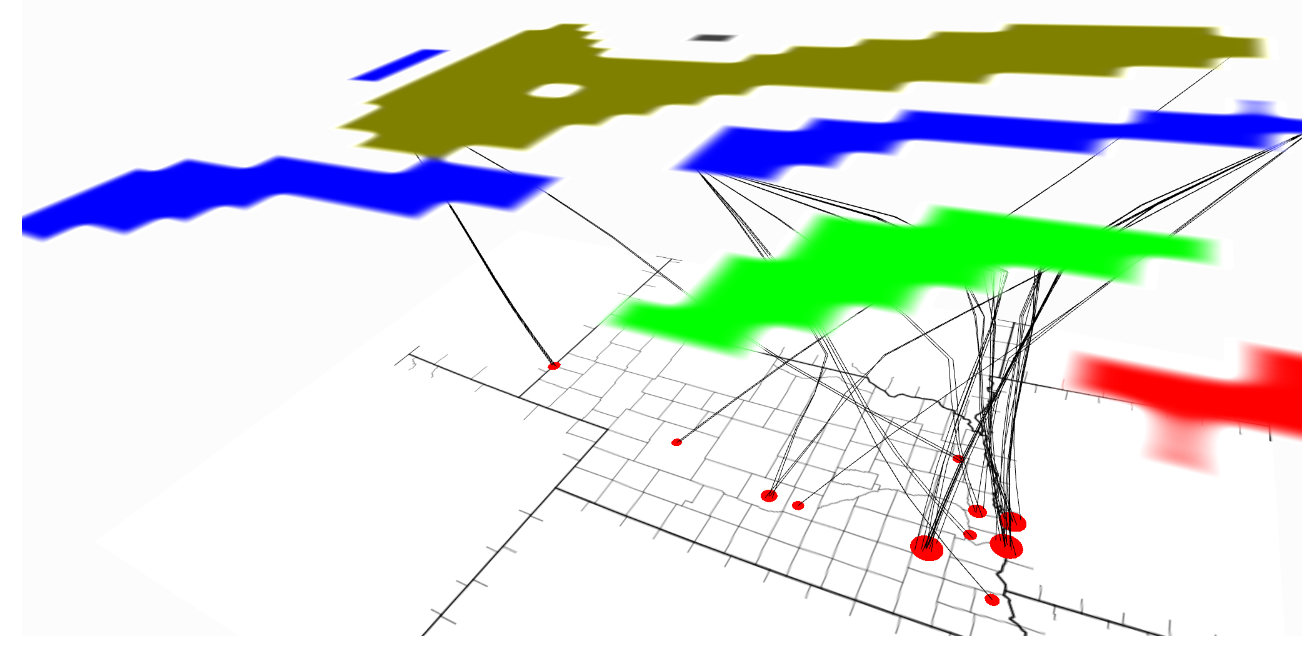
\includegraphics[scale=0.09]{blurBefore}}\quad
%  \subfigure[Secondary Cluster]{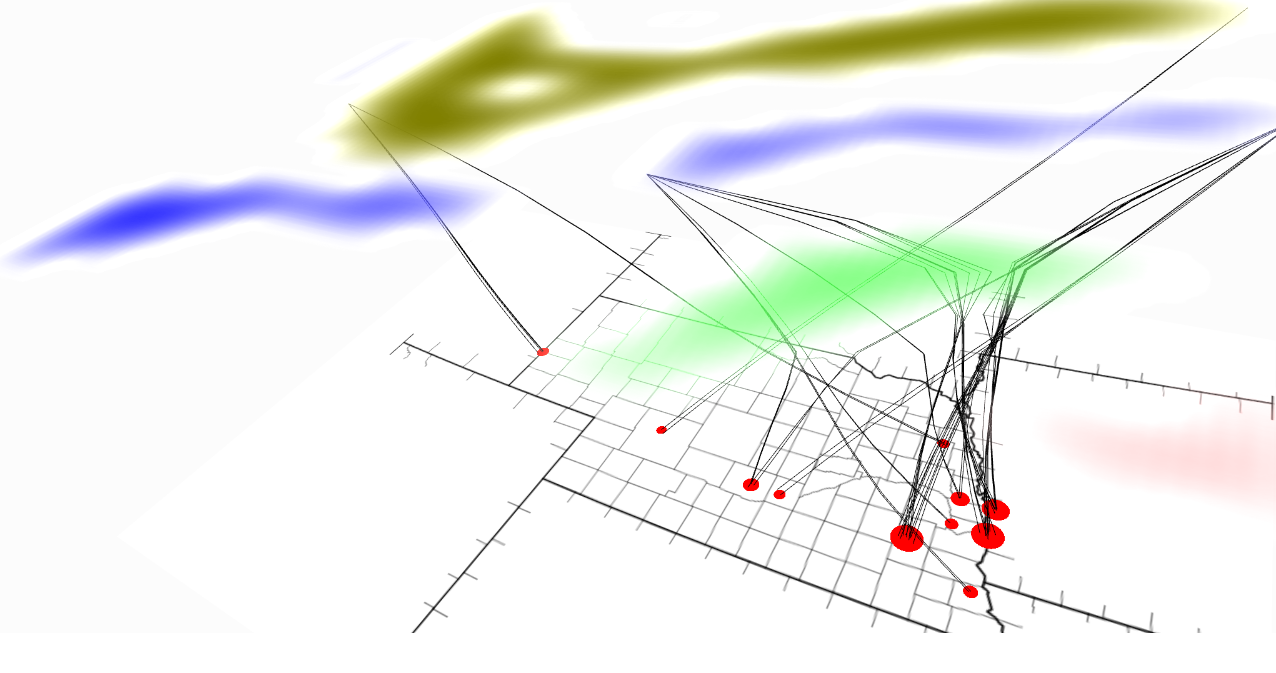
\includegraphics[scale=0.09]{blurAfter}}\quad
%  \subfigure[Tertiary Cluster]{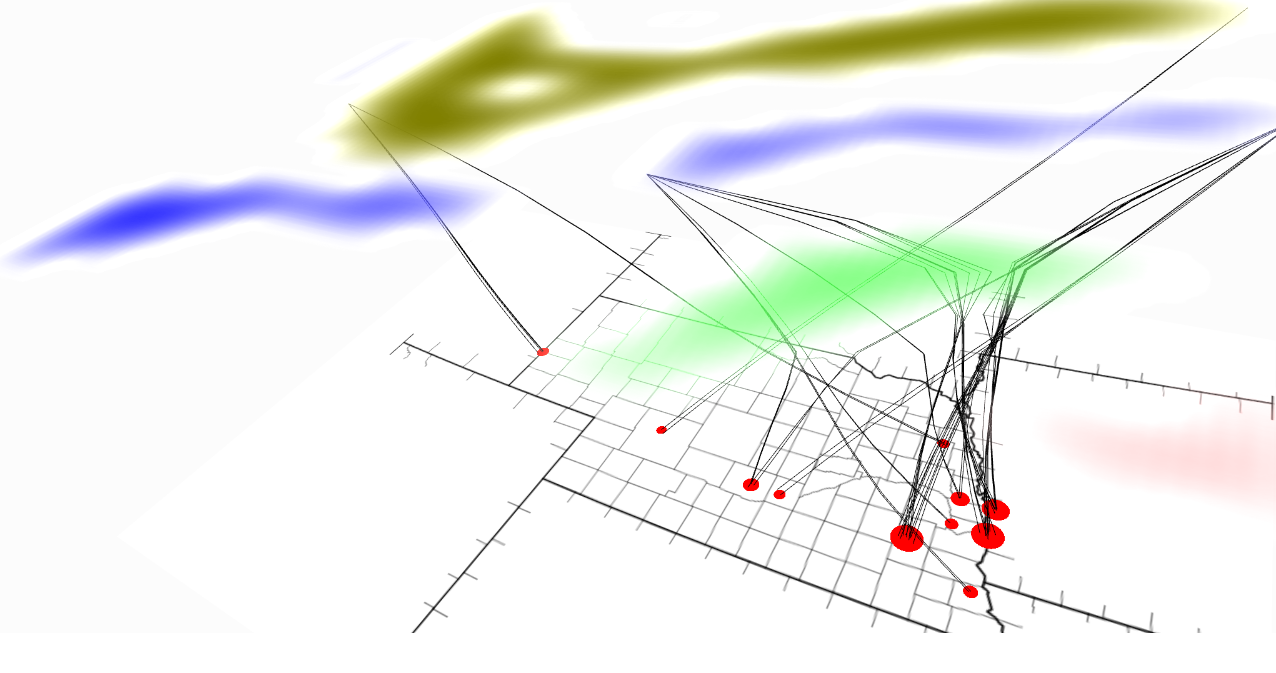
\includegraphics[scale=0.09]{blurAfter}}
%\caption{Clustering of the weather. In this hour, we see five different clusters. The blue cluster is seen in three different locations.}
%\label{fig:clusters}
%\end{figure}
%%------------------------------------------------

\section{Prediction}
\label{sec:pred}

Predicting the future is mostly based on facts. We have at our disposal the current mood and the current temperature, all of the previous days tweets and the temperatures for each hour, and the predicted temperature for each hour for the next two days. Using these facts, we try to determine what the sentiment at each tweet location will be for the next two days.

Determining the mood of the current locations up to 72 hours in the future is non-trivial. Our prediction technique is based on the current hour and the previous day. We choose not to use data from earlier times because the trends today are definitely not the same a year ago, let alone a month ago. In addition to this, we should state that the long-term weather is relatively unpredictable for the state of Nebraska.

%We start with the most rudimentary implementation, by solely comparing which number is closer by simply comparing the difference.
We start with a simple method of only comparing the TSK difference. If the current temperature is closer to the predicted temperature, we use the sentiment for the current hour to show the prediction. If the sentiment of the hour we are trying to pick has a closer temperature to the same hour of the previous day, we use the sentiment from the previous day.

%Seeing that the previously stated implementation was very crude, we tried a different method.
However, this simple method neglects the time. Alternatively, we can consider the time difference and state that if the current hour is closer to the predicted hour we will place a higher weight on using the current hours values; when the current hour goes further from the predicted hour, we can place more weight on the previous day value. %That is the further we are from the current hour the less weight it plays.
Using this method we take the sentiment based on the percentage of the weight in terms of time.

%The final method we use is a combination of above methods. We first determine the closest temperature value to the hour we are trying to predict the sentiment. Then, based on the difference, we determine the weight the two different sentiment sets place \eqref{eq:w}. As we see in \eqref{eq:p} X and Y represent the current temperature and the previous day's temperature respectively, and Z represents the temperature of the hour that we are trying to predict. The number of good and bad sentiment lines is calculated in \eqref{eq:gb}, where $G$ and $B$ represent the number good and bad tweets predicted by using the good and bad tweets of X and Y. The details regarding how well the different methods performed will be seen later on in the case studies.

%------------------------------------------------
\begin{figure}[t]
\begin{center}
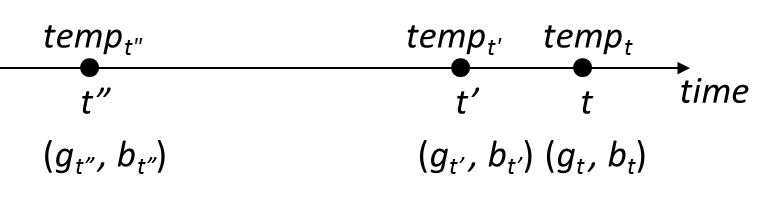
\includegraphics[width=0.8\linewidth]{predict}
\end{center}
\vspace{-.1in}
\caption{The prediction model.}
\label{fig:predict-model}
\end{figure}
%------------------------------------------------

%------------------------------------------------
\begin{figure*}[t]
\begin{center}
$\begin{array}{c@{\hspace{0.01\linewidth}}c@{\hspace{0.01\linewidth}}c}
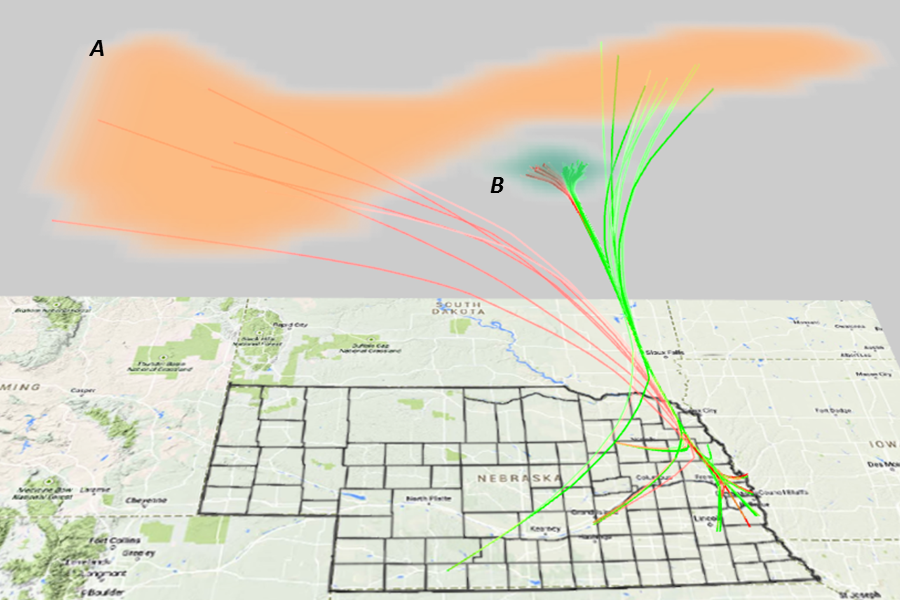
\includegraphics[width=0.33\linewidth]{endpoints_1} &
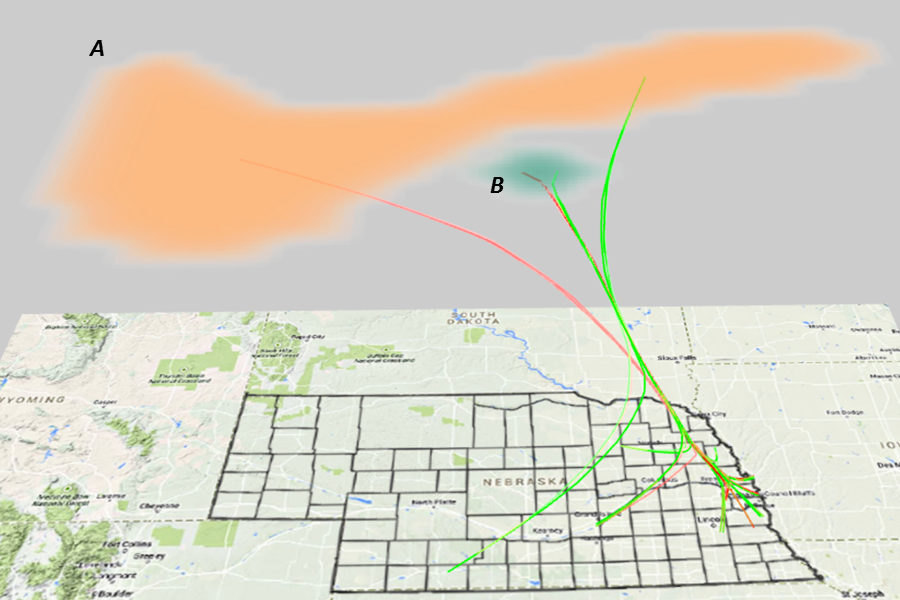
\includegraphics[width=0.33\linewidth]{endpoints_2} &
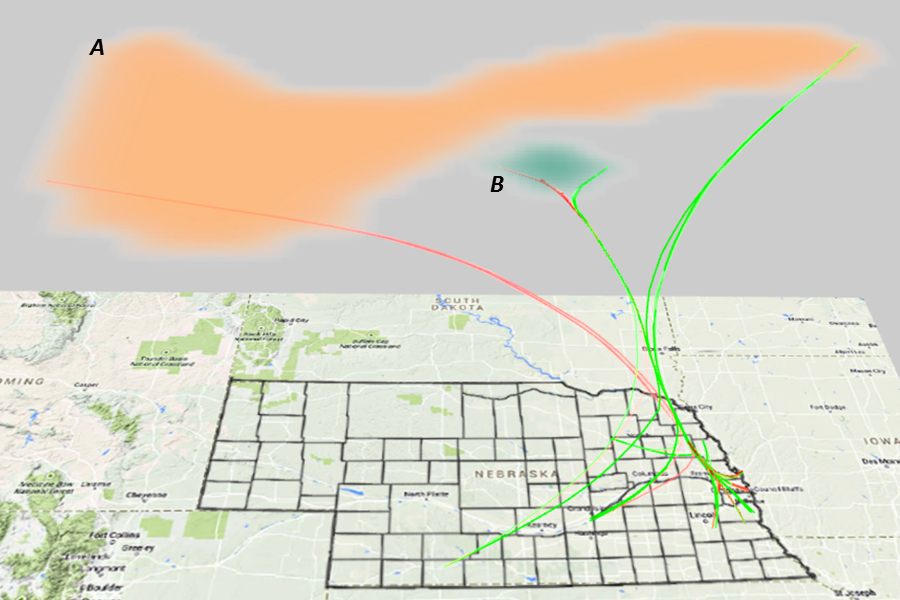
\includegraphics[width=0.33\linewidth]{endpoints_3}
\\
\mbox{\small{(a)}} & \mbox{\small{(b)}} & \mbox{\small{(c)}}
\end{array}$
\end{center}
\vspace{-.1in}
\caption{Determining the best positions for indicating negative and positive tweets in the cloud repressions of clusters. (a) Use the different point of a cluster for each edge. It can easily generate visual clutter. (b) Use the center points of the two halves of a cluster. This method is effective for a large cluster $A$, but makes it difficult to distinguish lines for a small cluster $B$. (c) Use the top rightmost point and  the bottom leftmost point of a cluster. This method is effective for both the large and small clusters, $A$ and $B$, respectively.}
\label{fig:corners}
\end{figure*}
%------------------------------------------------

The final method we use is a combination of above methods. As shown in Figure~\ref{fig:predict-model}, we want to predict the sentiments at a future hour $t$, and we have the following information:
%
%----------------------------------------------------------
\begin{itemize}
\vspace{-.1in}
\setlength{\topsep}{-0.1in}
\setlength{\itemsep}{-0.05in}
\item $t'$ is the current hour;
\item $t''$ is the same hour as the predicted hour on the previous day, i.e., $t'' = t - 24$;
\item $temp_t$, $temp_{t'}$ and $temp_{t''}$ are the TSK values at $t$, $t'$, and $t''$, respectively;
\item $g_{t'}$ ($g_{t''}$) is the total number of tweets with positive emotions at $t'$ ($t''$) correlated to the clusters of $temp_{t'}$ ($temp_{t''}$);
\item $b_{t'}$ ($b_{t''}$) is the total number of tweets with negative emotions at $t'$ ($t''$) correlated to the clusters of $temp_{t'}$ ($temp_{t''}$).
\end{itemize}
\vspace{-0.05in}
%----------------------------------------------------------
%
Based on this information, we first compute the differences between the TSK values:
%
%----------------------------------------------------------
\begin{equation}
\label{eq:p}
p_{t'}=\left | temp_t - temp_{t'} \right |;	\qquad p_{t''}=\left | temp_t - temp_{t''} \right |	
\end{equation}
%----------------------------------------------------------
%
According to the difference values, $p_{t'}$ and $p_{t''}$, we determine the weights of the two sentiment sets:
%
%----------------------------------------------------------
\begin{equation}
\label{eq:w}
w_{t'}=\frac{p_{t''}}{p_{t'} + p_{t''}}; 	\qquad w_{t''}=\frac{p_{t'}}{p_{t'} + p_{t''}}
\end{equation}
%----------------------------------------------------------
%
Finally, we estimate the amount of tweets with positive and negative emotions, $g_t$ and $b_t$, at $t$ with respect to $temp_t$ as:
%
%----------------------------------------------------------
\begin{equation}
\label{eq:gb}
g_t = g_{t'}w_{t'} + g_{t''}w_{t''};	\qquad b_t = b_{t'}w_{t'} + b_{t''}w_{t''}	
\end{equation}
%----------------------------------------------------------
%
The method accounts directly for both the time and the temperature. We will demonstrate the details regarding how well these three methods in Section~\ref{sec:caseprediction}.

%We first determine the closest temperature value to the hour we are trying to predict the sentiment. Then, based on the difference, we determine the weight the two different sentiment sets place \eqref{eq:w}. As we see in \eqref{eq:p} X and Y represent the current temperature and the previous day's temperature respectively, and Z represents the temperature of the hour that we are trying to predict. The number of good and bad sentiment lines is calculated in \eqref{eq:gb}, where $G$ and $B$ represent the number good and bad tweets predicted by using the good and bad tweets of X and Y. The details regarding how well the different methods performed will be seen later on in the case studies.
%
%$p_1$ and $p_2$ represent the difference between the temperatures
%\begin{equation} \label{eq:p} p_{1}=\left | Z-X \right |	\qquad p_{2}=\left | Z-Y \right |	 \end{equation}
%
%$w_1$ and $w_2$ represent weight of the temperatures
%\begin{equation} \label{eq:w} w_{1}=\frac{p_{2}}{p_{1}+p_{2}} 	\qquad w_{2}=\frac{p_{1}}{p_{1}+p_{2}}   \end{equation}
%
%$g_x, g_y, b_x,$ and $b_y$ represent the amount of good and bad tweets in X and Y
%\begin{equation} \label{eq:gb}  G = g_{x}w_{1} + g_{y}w_{2}	\qquad B = b_{x}w_{1} + b_{y}w_{2}	 \end{equation}




\section{Visualization}
\label{sec:vis}

We design a novel 3D visualization to picture the analytics of weather clustering, sentiment classification, and the corresponding correlation and prediction. The visualization is comprised of multiple layers, and there is a natural visual connection between the layers such that the weather above affects the people below.
%Many different methods could represent this data correlation however, we have created a novel visualization where the weather above affects the people below.
The layers are connected via line bundles to dictate how the majority of the Twitter users in Nebraska are feeling. This visualization provides a novel and more intuitive way to present the data.

\subsection{Layers}

The visualization is represented by three main layers. The base layer contains the map of Nebraska and neighboring states. We have chosen to show the counties in Nebraska to gain insight on the population distribution in the state, and choose to keep the other states plain to indicate emphasis of correlation to Nebraska. 
%On the map of Nebraska, there are circles indicating the area that Twitter users are posting from. The radius of a circle corresponds to the amount of people posting tweets in the vicinity. 
Using the WRF data set for the longitude and latitude values for the map, we compute the values at intermediate locations via interpolation. We use the longitude and latitude location of each tweet to place it on the map.
%For each tweet location, the Euclidean distance is calculated to get the nearest longitude and latitude location.

The topmost layer shows the weather clusters by lifting each cluster vertically from its geographic region on the ground of map. We visualize the weather clusters using a cloud representation (Section\ref{sec:cloud}). The middle layer contains the edges which start from the Twitter user location and ends at the weather cluster they correspond to above, according to the correlation results. We use the edge bundling method to succinctly display the complex edges while suppressing visual clutter (Section~\ref{sec:line}).

\subsection{Cloud Representation}
\label{sec:cloud}

In our visualization, the weather clusters appear as clouds. Each cluster is blurred at the boundaries to make the graphical interface cleaner and aesthetically pleasing. The color of each weather cluster is mapped from indigo to dark orange with respect to lower and higher TSK values. Clusters which are not connected of the same color indicate the same conditions (i.e., similar temperature) as other locations of the state. %as seen in Figure \ref{fig:blur}.

Because each cluster can be possibly correlated to the tweets with positive and negative emotions, we need to locate two types of edge points in the cluster for the tweets to link up to. We explore three designs on how the points should be picked. First, we assign half of one cluster to the positive emotions and the other half to the negative emotions. This visualization can easily generate a cluttered output, as shown in Figure~\ref{fig:corners} (a). Second, we split a cluster in half and use the center points of the two halves. This method is effective until we come into situations where the cluster is represented by a very small amount of data points, causing a clutter visualization again, as shown in Figure~\ref{fig:corners} (b). Finally, we map the tweets with positive emotions to the top rightmost point of a cluster, and map the tweets with negative emotions to the bottom leftmost point of the cluster. This method can significantly reduce visual clutter and help in situations where the cluster size is fairly small, as shown in Figure~\ref{fig:corners} (c).
%Initially, we had the Twitter user space and the weather space flipped. However, we believe that the way we present the data is novel and more intuitive.


%\begin{figure}[t]
%  \centering
%  \subfigure[Before blurring]{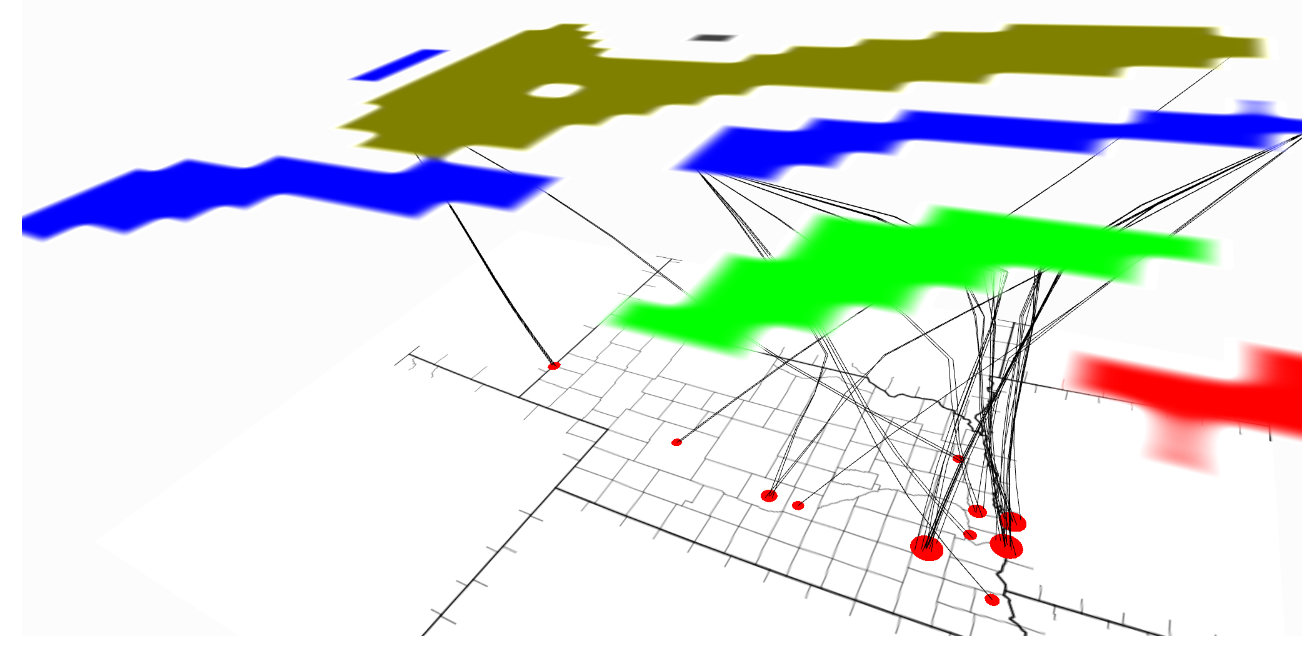
\includegraphics[scale=0.09]{blurBefore}}\quad
%  \subfigure[After blurring]{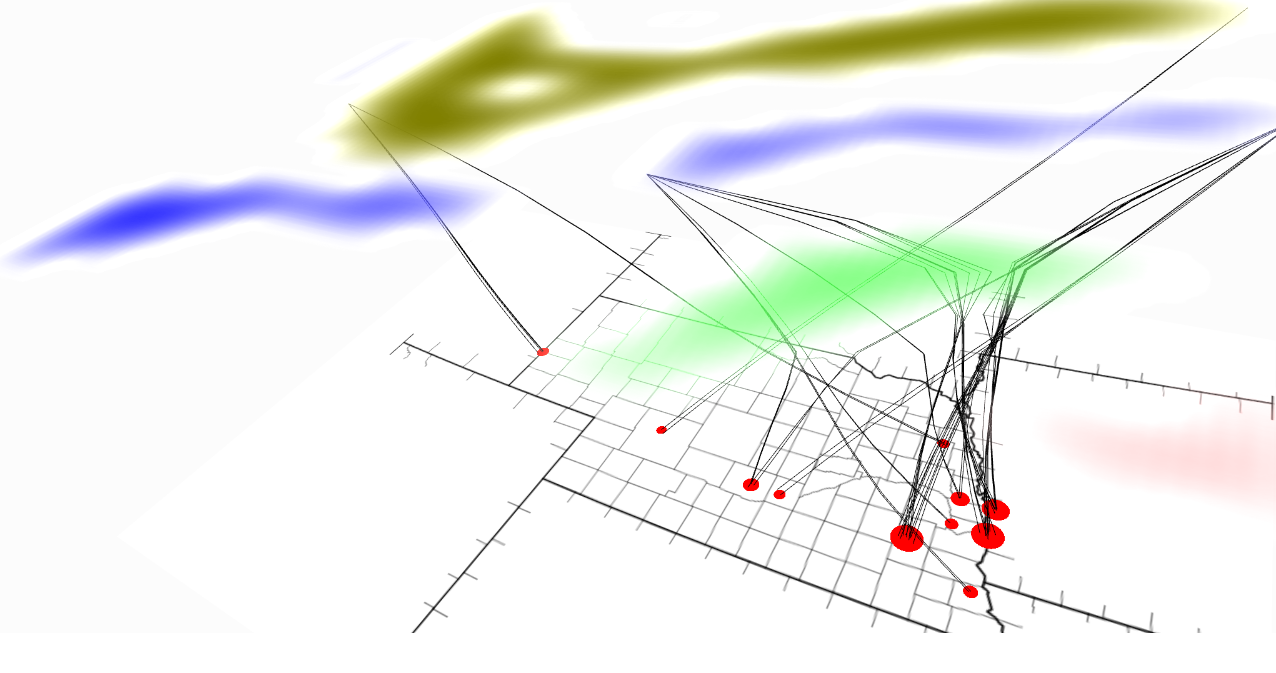
\includegraphics[scale=0.09]{blurAfter}}
%\caption{Clustering of the weather. In this hour we see five different clusters. The blue cluster is seen in three different locations.}
%\label{fig:blur}
%\end{figure}

%\begin{figure*}[htp]
%  \centering
%  \subfigure[Half good half bad]{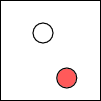
\includegraphics[scale=1.5]{sample}}\quad
%  \subfigure[Half good half bad centers]{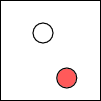
\includegraphics[scale=1.5]{sample}}\quad
%  \subfigure[Corners]{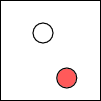
\includegraphics[scale=1.5]{sample}}
%\caption{Determining the best position for indicating negative and positive tweets in the cloud clusters.}
%\label{fig:corners}
%\end{figure*}


\subsection{Edge Bundling}
\label{sec:line}




Our design naturally forms a graph to represent the correlation between weather and tweets. However, visual clutter can easily occur if we directly display each edge as a straight line, as shown in Figure~\ref{fig:compareline} (a).
%
To address this issue, we adopt FDEB~\cite{holten2009force} to visualize the graph of correlation. We bundle the related edges with high compatibilities, and iteratively subdivide the edges to generate smooth curves with coherent shapes. This method can effectively reduce visual clutter in 3D.

The original paper of FDEB~\cite{holten2009force} proposed four criteria, angle, scale, position, and visibility, for edge compatibility measures. In our design, as the edges are mostly oriented along the vertical direction between cloud and ground, the variation in angle or scale is relatively marginal compared to a general graph. In addition, as we display the edges in 3D, the visibility of an edge can be changed from different views. Therefore, only position (i.e., distance between midpoints of edges) is considered for computing edge compatibility in our design.

%------------------------------------------------
\begin{figure}[t]
\begin{center}
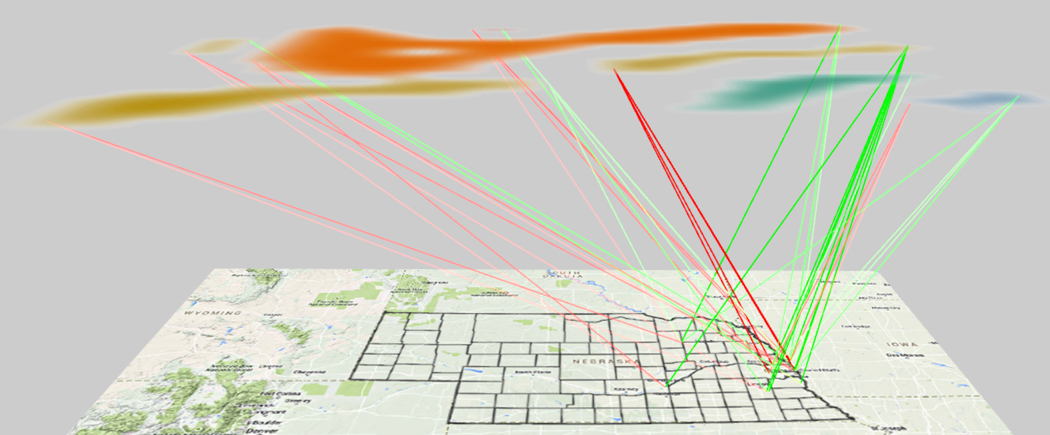
\includegraphics[width=0.75\linewidth]{edge_line} \\
\mbox{\small{(a)}} \\
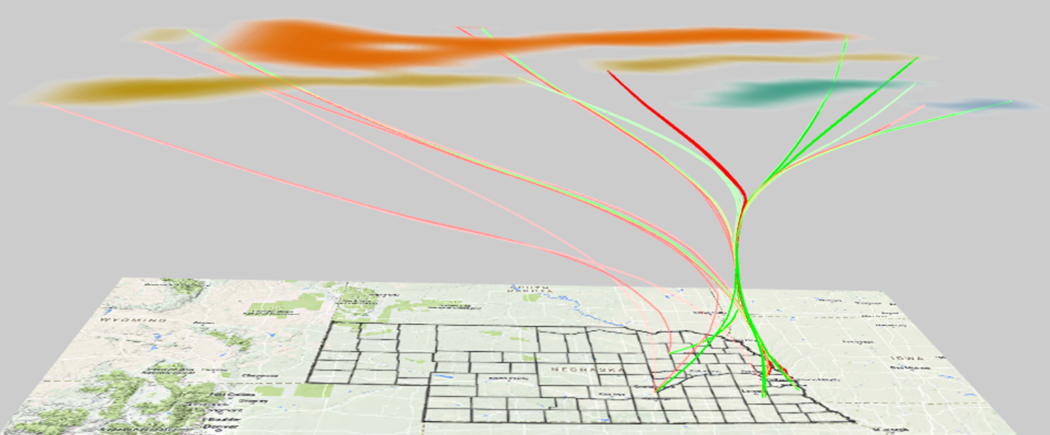
\includegraphics[width=0.75\linewidth]{edge_bundle} \\
\mbox{\small{(b)}}
\end{center}
\vspace{-.1in}
\caption{(a) A direct visualization of the correlation graph. (b) The edge bundling result.}
\label{fig:compareline}
\end{figure}
%------------------------------------------------

%------------------------------------------------
\begin{figure}[t]
\begin{center}
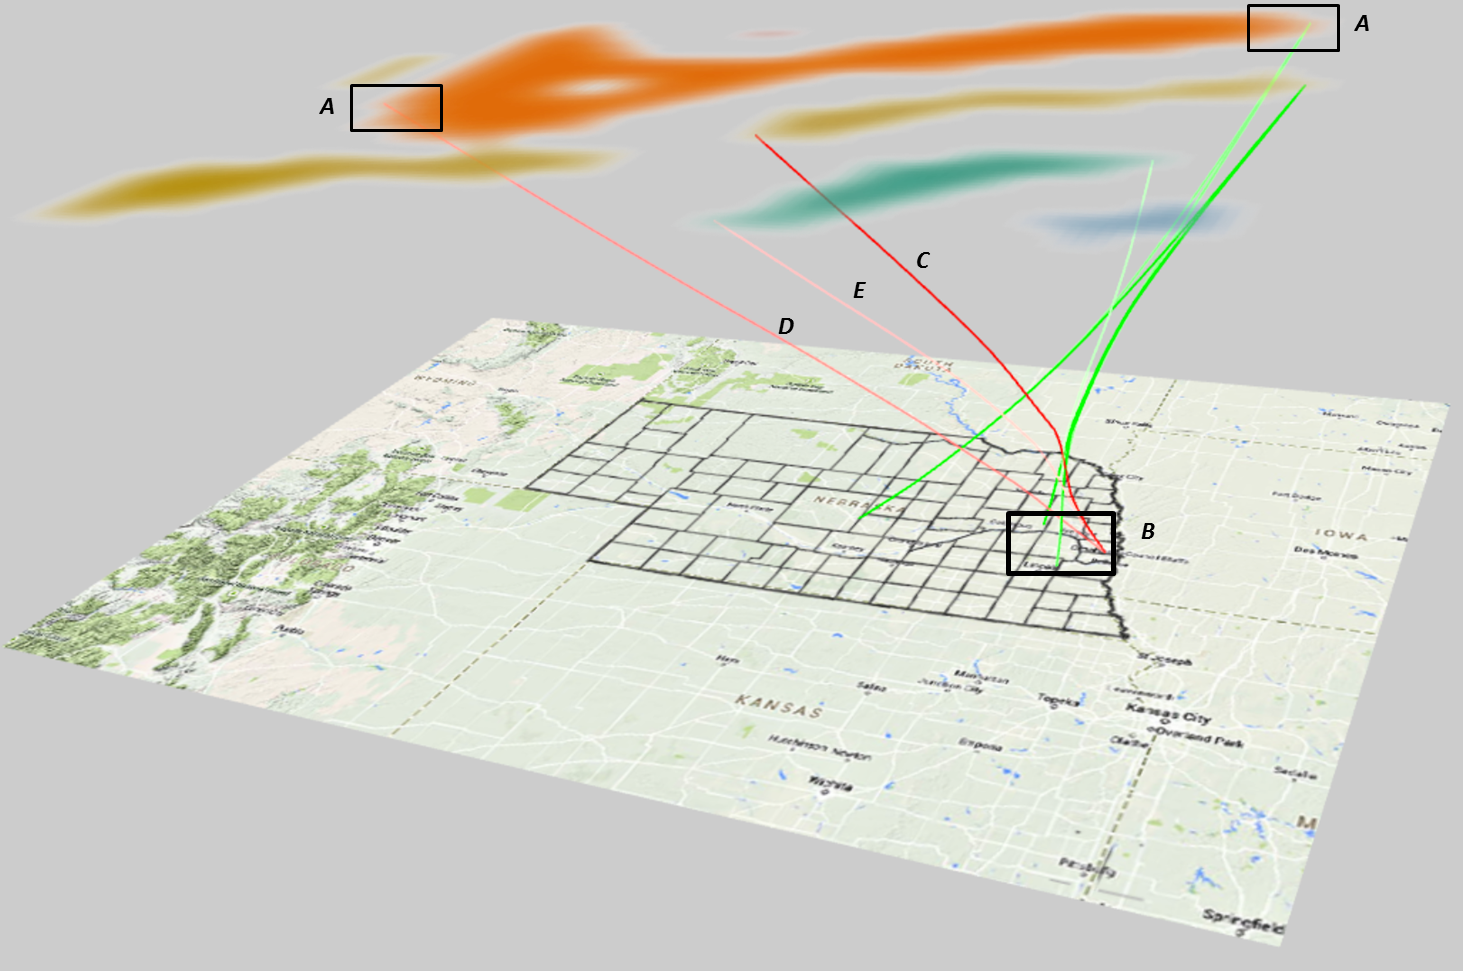
\includegraphics[width=0.75\linewidth]{bundle_details}
\end{center}
\vspace{-.1in}
\caption{The detailed configuration of line bundles.}
\label{fig:linedetail}
\end{figure}
%------------------------------------------------

Similar to FDEB, we use an iterative simulation to refine the bundling. The simulation starts with $P_0$ subdivision points for each edge, and then performs $C$ simulation cycles. During each cycle, a specific number of iteration steps $I$ is conducted to move the subdivision points to reach an equilibrium between forces. The number of iteration steps during the first cycle is $I_0$. After performing a cycle, the number of subdivision points is doubled to smoothen the edges, and the number of iteration steps $I$ is decreased by a factor $R$. We found that a configuration of $P_0=1$, $C=6$, $I_0=50$, and $R=\frac{2}{3}$ leads to appropriate results in our design. Figure~\ref{fig:compareline} (b) shows the edge bundling result of the same graph as in (a).

Each bundle is composed of multiple lines where each line represents one tweet. Every line corresponds to a positive or negative sentiment. The sentiment is represented in two ways. First, from the weather cluster perspective, we indicate the sentiment according to which corner of a cluster the bundle is linked to. In this way, we can easily examine the sentiments affected by a certain cluster, as shown in the two highlighted boxes as in Figure~\ref{fig:linedetail}. Second, from the tweet perspective, we associate the positive sentiments to the green bundles and the negative sentiments to the red bundles. In this way, we can intuitively convey the sentiments distribution among the tweets, as shown in the highlighted box B in Figure~\ref{fig:linedetail}.

The opacity of each bundle represents the intensity of the correlation between the cluster and the tweets. The bolder the line the stronger the relationship between the two points is. The primary cluster has a stronger hue in comparison to the secondary and tertiary clusters. These links associated with the secondary and tertiary clusters have a staggered decrease of intensity of color. Thus, we state that the more prominent the link between the tweet and the cluster the higher the opacity of the line. The lines C, D, and E in Figure~\ref{fig:linedetail} show an example of the opacity values of lines associated with the primary, secondary, and tertiary clusters, respectively.



\section{Case Studies}

For our work, we have two goals. We first want to determine if there is any correlation between weather and mood. Secondly we would like to determine if our predicted mood is correct.

\begin{figure*}[htp]
  \centering
  \subfigure[Temperatures in Omaha and Lincoln]{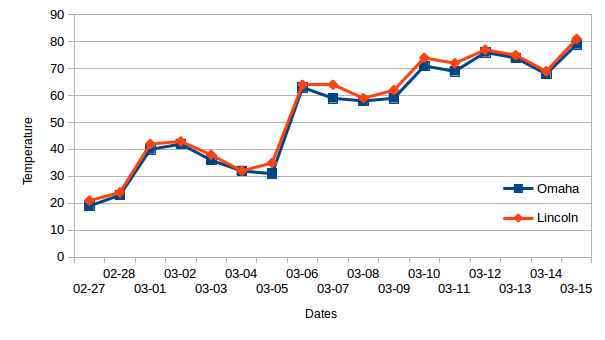
\includegraphics[scale=0.25]{chart1}}\quad
  \subfigure[Sentiment of Omaha and Lincoln Tweets]{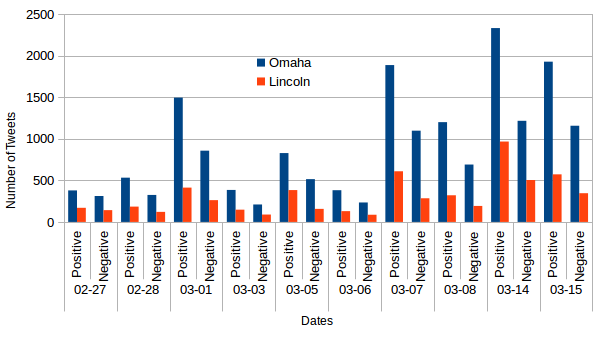
\includegraphics[scale=0.25]{chart2}}\quad
  \subfigure[Sentiment of Omaha and Lincoln Tweets]{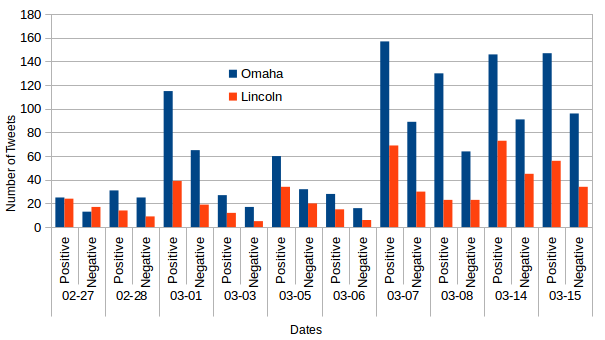
\includegraphics[scale=0.25]{chart3}}
\caption{The comparison of weather to sentiment.}
\label{fig:chart_1}
\end{figure*}



\subsection{Tweet weather correlation}
We use two data sets to show our visualization. Using weather and twitter data from two back to back weekends we see if there is any relationship between the temperature and the overall mood of people. We are lucky that the days we chose show warmer changes in weather. Being on the brink of Spring we predict that the overall Tweets for the warmer weekend will have a more positive sentiment in comparison to the colder weekend. This weather pattern also can show any correlation we find for seasonal affective disorder (SAD)~\cite{denissen2008effects}.

\subsubsection{All Tweets}
Of all the cities, we see that Omaha and Lincoln have the most tweets, so we will use these two cities to display our results. The weather patterns of the two weekends are shown in Figure \ref{fig:chart_1}(a). As seen in the figure, we choose to look at times where most of the population is awake (i.e. noon to 11 PM). From Figure \ref{fig:chart_1}(b) we can see the tweets and their sentiment for select days through the two weeks, where more emphasis is placed on the first week and less on the later. Each date has a positive and negative count, where we see that the pattern throughout is that the positive tweets outweigh the negative tweets. Another pattern that we see is that as the temperature increases the number of tweets increase however we see that more people tweet on Saturday than on Sunday. We think that this has to do with a number of factors; people go to church on Sunday where they choose to be among family, they do work around the house, or they don't have any eventful things which they feel they need to share.

We do not see that with the change of temperature that there is a clear trend of more positive tweets versus negative tweets. The number of positive tweets is at least half the amount of negative tweets. The only item that we could see which may be weather related is that the amount of negative tweets is percentage wise far more in the colder temperatures in comparison to the warmer temperatures. In lieu of not finding any clear results, we look at tweets only with words related to weather to see if we find any trends.



\subsubsection{Weather related tweets}

Other than using all the tweets we collected we filter the collected tweets for weather-related terms. (i.e. snow, sunny, warm, cold, rain, etc.) We wanted to see if there was a stronger correlation in this situation compared to using all the tweets collected. In this situation, we are unfortunately limited to a few tweets. As we see in Figure \ref{fig:chart_1}(c) we see that the number of tweets drastically reduces to at most slightly less than 160 tweets for one day.

Fortunately, we are able to see a pattern with weather and positive tweets. There is a spike of tweets when there is warmer weather. This pattern is seen in both sets of tweet data sets. However, we are now able to confirm that the correlation is due to weather. As the weather increased slightly on March 1st we see a spike in amount of tweets overall(Figure \ref{fig:chart_1}(b)) and also when the tweets had weather-related words(Figure \ref{fig:chart_1}(c)). We can also see that in Figure \ref{fig:chart_1}(c) that with the warmer weather the number of tweets in relation to the weather increased by approximately twice the amount. We still see the trend of more positive tweets in comparison to negative tweets when using the filtered data set.

\begin{figure}[htb]
 \centering
 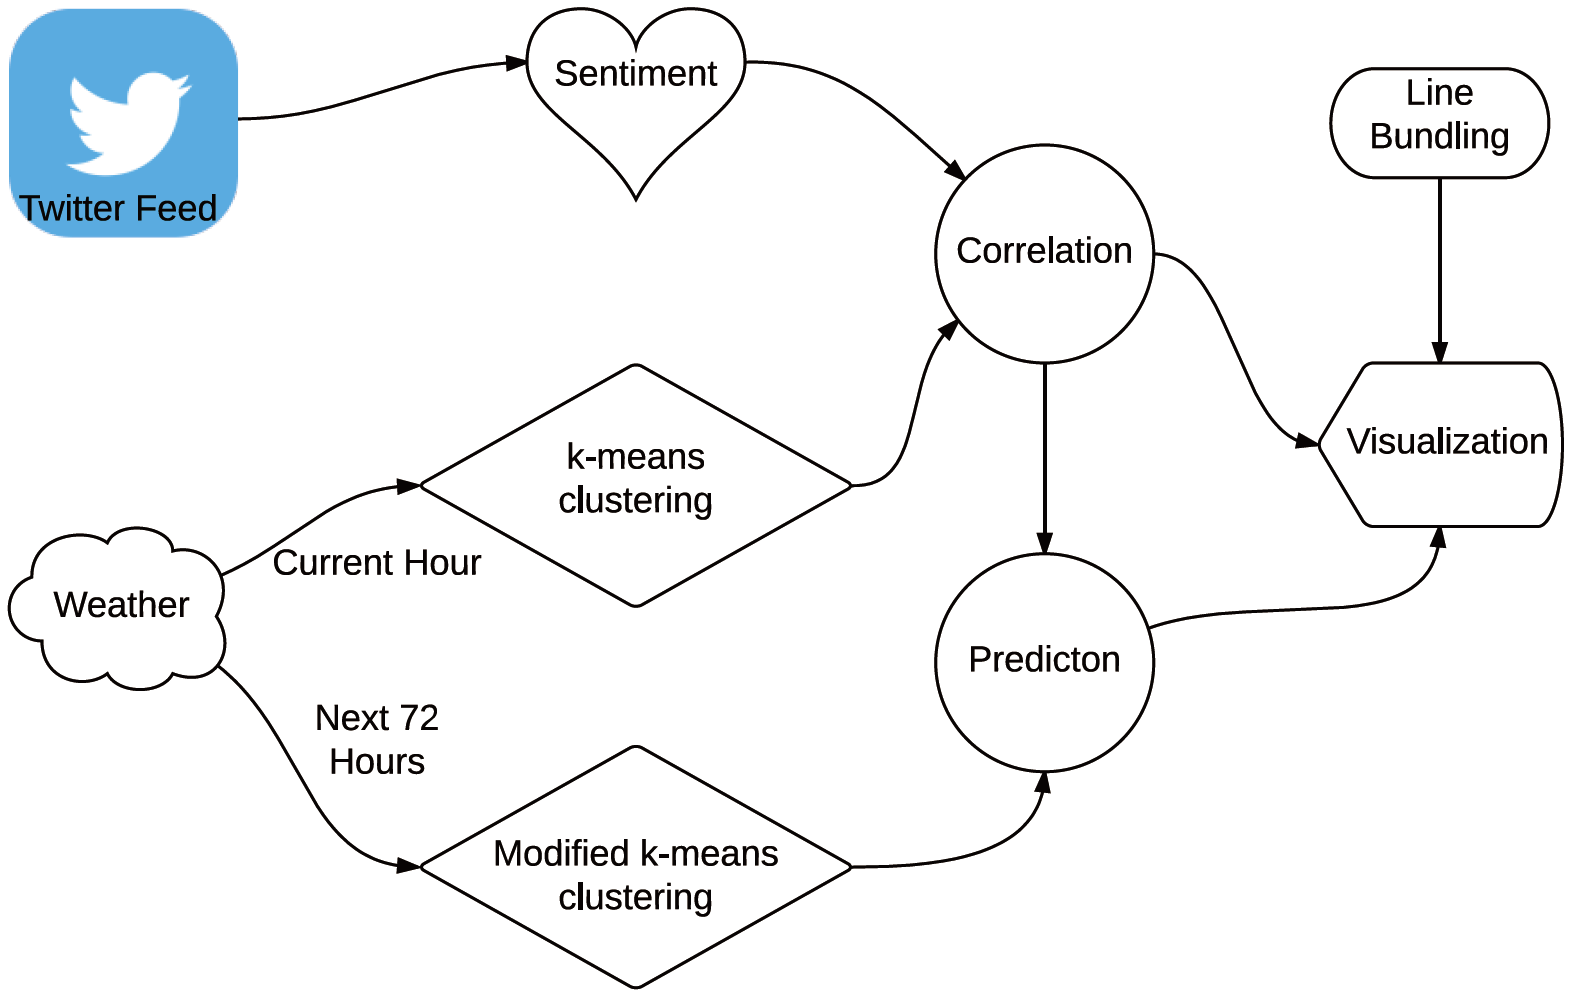
\includegraphics[scale=0.1]{steps}
 \caption{Accuracy of the different prediction methods}
 \label{fig:predict}
\end{figure}

\subsection{Predicted?}
Using the same data set we select a subset of two weekends to determine if the predicted value was close to the outcome. We chose March 6th, 7th and 8th for weekend one and March 13th, 14th and 15th for weekend two. The first weekend has between 10 to 20 degrees difference to the second weekend to take into account any change in weather patterns. We collect our predictions for Saturday and Sunday and compare them to the real sentiment of each hour. Again we focus on the two most populous cities in Nebraska; Lincoln and Omaha.

As we see in Figure \ref{fig:predict} the accuracy of the three methods we used are shown.


\chapter{Discussion}

%We used the large data set to determine if there was any noticeable correlation, and we filter the data set to determine if this could provide a better indication of correlation. We saw that most of the tweets were positive in colder and warmer temperatures, however, the number of tweets increased as the temperature rose. We observed the number of positive tweets percentage wise was much higher when the temperature rose. Even though, our initial aim was to find a distinct answer to the question: Does the weather affect mood?, we were not able to gain concrete results. We were able to find other patterns from our analysis.
%
%We were able to determine the possible sentiment of users in select regions, even with lower a population. The results show ......
%
%Correlating tweets to weather patterns is not a trivial task and requires multiple steps which can create errors at each step. Having a multi-step process the chance of error from classification can occur.

There are a few aspects in regards to tweets that enforces a limit as to what we can assess. One limitation from tweets is that with a state population as small as Nebraska the chance of a user with their location enabled is relatively low. This limits the amount of tweets we can attain each hour. Tweet length imposes another limitation because the complete expression of a user's feelings can be curbed in some situations. Other than Twitter's limits we need to examine the suppressed feelings of users. As Twitter is a social media hub, the need to express oneself in 140 characters may place a mask to what the user may be feeling. As proposed before there is no distinct way to determine the true feelings of a person~\cite{hannak2012tweetin}. Given this phenomena, we experimented the usage of only weather related tweets because there is a lower chance of users masking their emotions. Even in this case we saw that the majority of users use their tweets in a positive manner, so to expect a negative tweet is cynical in some sense.

Classifying the sentiment always brings errors. Humans are not known to be the most accurate at identifying the sentiment of written statements~\cite{pangthumbs}. %When bringing in our own classifier, we believe that it can be improved. 
There are always certain words that can make the sentiment have a positive value instead of negative. Tweets are known to have sarcasm in terms of introducing a form of satire or irony~\cite{riloff2013sarcasm}. In situations like this there are some misclassifications of sentiment.

%We believe that using the current weather limits us on other seasons which are approaching. So far, 
We have experienced winter and spring weather in our current study. When we have the change of seasons it is easy to see that there is some correlation with SAD. Like most of the population, the end of winter brings new changes, and thus new feelings. We will study the sentiment changes when summer, fall, or winter approaches. Nebraska is known for its intense heat and harsh winters, but these seasons also entail vacations and family gatherings. Analyzing these aspects can also provide more insight regarding our data sets and other filtering processes that we may need.

\chapter{Conclusion}

In this work, we have presented a 3D visualization tool, named Tweether, that can assist analysts to explore the correlation of weather to tweets in geospace and time. We extract the dominant patterns from the weather data and classify the sentiments from the synchronized tweets. We identify the relation between weather and tweets using their geospatial relationship and the Pearson product-moment correlation coefficient. We tailor FDEB to our layered visual design and employ line bundles to show detailed graphs of the connection between the weather clusters and the tweets. With a fine tune on graph vertex placement and edge properties, our line bundling can significantly reduce visual clutter and clearly reveal the sentiment distribution with respect to different weather conditions in 3D. In addition, we develop a prediction model to estimate the future emotions among the tweets according to the forecasted weather. Our Tweether system integrates these data analysis models and interactive visualization, and facilities users to visually examine the connection between weather and mood and identify a possible relationship.
%
Although researchers have presented visualizations showcasing social media sentiment or clustering of weather patterns, to the best of our knowledge we have presented here the first application to visualize the correlation between the two.

%Our case study has revealed some discoveries between temperature and moods
%such as there is correlation with the amount of tweets related to weather when it is warm in comparison to the colder weather,
%that have been justified in other research areas~\cite{keller2005warm}.

The future of this research can be expanded immensely. Although we focus on the relation to temperature in this work, the general design philosophy can be applied to precipitation, humidity, wind speed, or any other weather variables.
%As we approach warmer climates
We will conduct research regarding what the overall sentiment of people to rain, storms, and strong wind conditions. For example, there may be a significant correlation between rain amount and negative tweets~\cite{hannak2012tweetin}. We also believe that we can determine if there is a better correlation of weather to other social phenomena or events, such as road accidents, calamities from natural disasters, or even medical episodes like the flu, which can be directly impacted by the weather. Given the possible uncertainty when determining if a person's mood is truly affected by weather, we plan to involve other social phenomena or events to obtain more concrete correlation results.
%
This work can be also expanded to other states. The outcomes in more populous states may be different. We are also interested in the states which experience less seasonal changes, and study the corresponding correlation between weather patterns and sentiment.

Other than visualization we would like to improve sentiment classifier by mining large tweet data to gain information regarding new words, such as determining sarcasm, irony, or satire, and find new linguistic patterns. This can also help improve the sentiment prediction.

%However, there have been few to none works that attempt to find the correlation between the two.

%the sentiment classification  and show detailed graphs of their connected based on FDEB.
%
%
%With a novel visualization to convey the connection between weather and sentiment in space and time, we can explore the effects of weather patterns on the usage of social media.
%
%
%our main goal was to determine if there was any correlation between usage of social media and weather patterns. Using two data sets, we were able to determine that there is some correlation with the amount of tweets related to weather when it is warm in comparison to the colder weather.
%
%Visualizations showcasing social media sentiment has been done many times before, and similarly clustering of weather has been implemented numerous times before. However, there have been few to none works out there which try to find the correlation between the two.
%
%We realized that this work can be expanded to apply to many different scenarios, but we chose to apply it to a question that has been asked for centuries. ...
%
%Our prediction technique worked for...
%
%The line bundling implemented in this visualization is an entity on its own and should be applied to many different works. ...



%\section{Future Work}
%
%The future of this research can be expanded immensely. There are various aspects we can add to the existing work, or even alter the existing work. For altering existing work, we would like to in the future make a cleaner looking visualization. Currently, there seems to be some rigidness to the design where corners could be smoothed have a clearer indication of what places link up to where. We also feel that we can make the design more intuitive without adding additional elements. Other than visualization we would like to implement a better sentiment classifier. Just by polling more tweets and gaining information regarding new words, determining sarcasm, irony, or satire, and finding new linguistic patterns we believe we can gain a better classifier. Additionally we would also like to improve the sentiment prediction.
%
%For supplementing this work, we have a few items which we believe we can add. This work as of now only sees the relation to temperature, but this study could be extended to be applied to precipitation, humidity, wind speed, or any other weather variables. There may be a significant correlation between rain amount and negative tweets. As we approach warmer climates we can conduct research regarding what the overall sentiment of people to rain, storms, and strong wind conditions. We also believe that we can determine if there is a better correlation of weather to other variables, possibly ones which are directly impacted by weather such as road accidents, calamities from natural disasters, or even medical episodes like the flu. Since there is no real way to determine if a person's mood is truly affected by weather we think using some other variables can provide more concrete correlation results.
%
%This work can be expanded to other states and see if in more populous states the outcome would be more different. We also think that states which don't experience much seasonal change will have very different outcomes and not reflect any correlation between weather patterns and sentiment. 


%% backmatter is needed at the end of the main body of your thesis to
%% set up page numbering correctly for the remainder of the thesis
\backmatter

%% Start the correct formatting for the appendices
\appendix

%% Appendices go here (if you have them)

%% Bibliography goes here (You better have one)
%% BibTeX is your friend
\bibliographystyle{plain}
\bibliography{tweether}
%% Pull in all the entries in the bibtex file. Is is a useful trick to
%% check all your references.
\nocite{*}

%% Index go here (if you have one)

\end{document}
\endinput
%%
%% End of file `thesis-test.tex'.
